\clearpage
\subsection{粗糙表面的倒影}

把同一面镜子的粗糙度从零调到 $0.34$，再去看灯牌。原本轮廓清楚的灯条向四周散开。从同一个像素出发，有些反射方向能看到亮条，有些只看到黑框。假设四次取样给出的红通道分别是 $0,0,0,4$，平均值是 $1$。只算其中一次，很容易把这里画得过亮或过暗。一张图里许多像素各取一次，这种波动就成了可见的颗粒。

\begin{center}\small
\begin{tabular}{@{}ccc@{}}
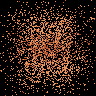
\includegraphics[width=.29\linewidth]{../../../output/profiling/rough-reflections/test-raw.png} &
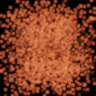
\includegraphics[width=.29\linewidth]{../../../output/profiling/rough-reflections/test-filtered.png} &

\includegraphics[width=.29\linewidth]{../../../output/profiling/rough-reflections/test-reference.png}\\[-1pt]
每个像素取一个方向 & 对左图的倒影降噪 & 每个像素取 512 个方向
\end{tabular}
\end{center}
{\small\color{quiet}Redflag 的 Vulkan 测试。左图的黑底上散着橙色亮点。中图使用同一次取样，单个亮点减少了，仍能看见大小不一的色块。右图用另外 512 个方向取平均，能看清上下两片较亮的倒影与中间稍暗的部分。三张图都用同一亮度显示。\par}

在粗糙度均匀的一小块平面上，相邻像素的位置和朝向相近，能收到的反射光往往也相近。左图已经为每个邻居算了一条反射光线。如果让中心像素借用几份这样的结果，一次恰好采到亮条所造成的误差就有机会减小。但镜面边缘紧挨着墙，或者材料突然从金属变为涂漆时，屏幕上再近的两个点也可能反射完全不同的颜色。

用 $p$ 表示中心像素，$q$ 表示附近的一个像素。记 $R(q)$ 为本次倒影给 $q$ 增添的线性 RGB。让越相近的表面在平均时占越大比重，把这个数叫作权重 $w(p,q)$。把每个 $R(q)$ 乘上它的权重，相加后再除以权重之和。这样即使有几个邻居落在墙面上而被排除，一块颜色均匀的镜面仍能保持原来的亮度。
\[
  \overline R(p)=
  \frac{\sum_{q}w(p,q)\,R(q)}{\sum_{q}w(p,q)} .
\]
举例说，三个像素的红通道是 $1,4,1$，权重分别取 $1,2,1$，得到 $(1+8+1)/4=2.5$。若第三个像素落在镜框上，它的权重改为零，分子与分母都要重新算，结果是 $(1+8)/3=3$。这组数字只为说明平均的算法。

实际计算时还要保住表面原有的照明。把计算倒影前的颜色记为 $B$，加上倒影后的颜色记为 $C$，就有 $R(q)=C(q)-B(q)$。着色器只对这份差值取平均，最后给它加回中心像素自己的 $B(p)$。这样即使相邻像素一个在阴影中、一个被灯直接照亮，它们的直接光仍各自留在原处。

在代码里，\texttt{ScreenEffects::Render} 先让 GPU 把 $C$ 写到一份单独的图里，再把它和原图 $B$ 一起交给降噪着色器。为了检查底图有没有被抹糊，测试把 $B$ 换成隔一个像素就换色的棋盘。用降噪后的图减去棋盘，再与黑底上的倒影逐像素比较，RGB 差值的长度最大仍小于百万分之一。\href{run:../../Redflag/src/Redflag/Renderer/ScreenSpace/ScreenEffects.cpp}{引擎调用}\quad\href{run:../profiling/rough-reflections/test-edges.csv}{棋盘与接缝读数}\quad\href{run:../profiling/rough-reflections/test-capture.json}{RenderDoc 的两次计算}

\clearpage
\subsection{相邻像素的取舍}

GPU 已经保存了相机看到的表面位置 $P$ 和法线 $n$。把两点间的位移 $P_q-P_p$ 沿中心法线 $n_p$ 投影，得到 $d=\lvert (P_q-P_p)\cdot n_p\rvert$。沿一块倾斜的平板移动时，点到相机的距离在变，两点的连线却始终贴着平板，$d$ 仍为零。如果邻点落在墙上，连线会离开平板，$d$ 随之增大。着色器沿邻点的法线也量一次，取两次中较大的距离。

\begin{center}
\begin{tikzpicture}[x=1mm,y=1mm,>=stealth, every node/.style={font=\small,text=ink}]
  \fill[wine!9] (5,3) rectangle (68,6);
  \draw[wine,very thick] (5,6) -- (68,6);
  \fill[ink!9] (87,14) rectangle (151,17);
  \draw[ink,thick] (87,17) -- (151,17);
  \draw[->,quiet] (25,6) -- (25,25) node[above]{中心法线};
  \fill[wine] (25,6) circle (.9) node[below=2mm]{中心 $p$};
  \fill[wine] (56,6) circle (.9) node[above=1mm]{同一平面};
  \draw[quiet,densely dashed] (68,6) -- (129,6);
  \fill[ink] (108,17) circle (.9) node[above=1mm]{另一表面 $q$};
  \draw[<->,wine] (121,6) -- (121,17) node[midway,right]{$d$};
\end{tikzpicture}
\end{center}
{\small\color{quiet}沿中心表面侧看。虚线延长了中心表面所在的平面。图中的 $d$ 是邻点到这个平面的垂直距离，按场景长度计算。\par}

靠近中心的邻居影响更大。横向从左到右的权重取 $1,4,6,4,1$，竖向也取这五个数，相乘便得到每个位置的权重。项目选了最多两圈邻居，粗糙度达到 $0.5$ 时才用满。两点沿法线分开的距离达到半个像素在场景中覆盖的宽度，或法线夹角达到约 $26^\circ$，权重就减到零。两点的底色或金属度差得太多也会分开计算。

\noindent{\small\color{quiet}按计算着色器 \href{run:../../Redflag/src/Redflag/Renderer/ScreenSpace/Shaders/ReflectionFilter.comp}{\texttt{ReflectionFilter.comp}} 整理的伪代码}\par\nopagebreak
\begin{lstlisting}[escapeinside={(*@}{@*)}]
if background(p) or perfectMirror(p): return color[p]
sumRGB = 0
sumWeight = 0
for q in nearbyPixels(p):
    w = sampleWeight(p, q)              (*@{\footnotesize\color{quiet}比较位置、朝向和材质。}@*)
    sumRGB += w * (color[q] - base[q])  (*@{\footnotesize\color{quiet}取邻居的倒影。}@*)
    sumWeight += w
return base[p] + sumRGB / sumWeight
\end{lstlisting}

在 $96\times96$ 的镜面上，把每个像素的红、绿、蓝与参考图对应的数值相减，平方后求平均。再对 16 帧取平均，就得到下表的均方误差。换成与前一帧相减，就能看出镜头固定时颜色还会波动多少。最后一列取亮条与灰条中央的红通道之差。\href{run:../../tests/RoughReflectionCheck.h}{测试代码}\quad\href{run:../profiling/rough-reflections/test-quality.csv}{读数}

\begin{center}\small
\begin{tabular}{@{}lrrr@{}}\toprule
同一镜面 & 对参考图的均方误差 & 相邻帧的均方差 & 灯条红通道差\\\midrule
每像素取一个方向 & \measured{rough-raw-mean_rgb_mse} & \measured{rough-raw-adjacent_rgb_mse} & \measured{rough-raw-bright_minus_middle_red}\\
倒影降噪后 & \measured{rough-filtered-mean_rgb_mse} & \measured{rough-filtered-adjacent_rgb_mse} & \measured{rough-filtered-bright_minus_middle_red}\\
参考图 & --- & --- & \measured{rough-reference-bright_minus_middle_red}\\\bottomrule
\end{tabular}
\end{center}

Dammertz 等人用位置和法线决定哪些样本可以一起平均，并逐轮拉开取样间距。Redflag 只对当前帧平均一次，小于取样范围的细纹仍可能被抹平。AMD 的反射降噪还会估算亮度波动，结合前一帧的颜色继续处理。
\href{https://jo.dreggn.org/home/2010_atrous.pdf}{HPG 2010，图 2、3 与式 (2)--(5)}\quad
\href{https://doi.org/10.2312/EGGH/HPG10/067-075}{论文 DOI}\quad
\href{https://gpuopen.com/manuals/fidelityfx_sdk/techniques/denoiser/}{AMD Denoiser 1.3}\quad
\href{https://github.com/GPUOpen-LibrariesAndSDKs/FidelityFX-SDK/blob/v1.1.4/sdk/include/FidelityFX/gpu/denoiser/ffx_denoiser_reflections_prefilter.h}{AMD 空间滤波源码}\quad
\href{https://pbr-book.org/4ed/Monte_Carlo_Integration/Monte_Carlo_Basics}{PBRT 第四版 §2.1.4，均方误差}
